%%
%  ******************************************************************************
%  * #file    Szablon_raportu_EN_Latex.tex
%  * #author  Adrian Wójcik   adrian.wojcik(at)put.poznan.pl
%  *          
%  * #commit  Patryk Kościk   koscikpatryk(at)gmail.com
%  *          Modified the template for Projekt przejsciowy purposes          
%  *          
%  * #version 1.0
%  * #date    09-Mar-2022
%  * #brief   PROJPRZEJ
%  *
%  ******************************************************************************
%%  
\documentclass[11pt, a4paper]{article}

\usepackage{SM_template}

% Wypełnijcie te dyrektywy zgodnie z waszym tematem
% \lab      -> NAZWA CZUJNIKA, np.: 'DHT22'
% \comment  -> Króciutki opis co to, np.: 'Cyfrowy budżetowy czujnik temperatury'
%
\lab{Moduł GY-521}
\comment{Moduł 6DOF z 3-osiowym akcelerometrem i 3-osiowym żyroskopem}

% Absolutny zakaz dotykania tego tutaj bo jak dotkiecie to coś jebnie
\university{Politechnika Poznańska}
\faculty{Wydział Automatyki, Robotyki i Elektrotechniki}
\institute{Instytut Robotyki i Inteligencji Maszynowej}
\department{Zakład Sterowania i Elektroniki Przemysłowej}
\addbibresource{bib/GY-521.bib}
\nocite{*}


%%
%
% Początek dokumentu
%
%%
% \vspace{0.3cm}
% \begin{figure}[H]
% \centering
% 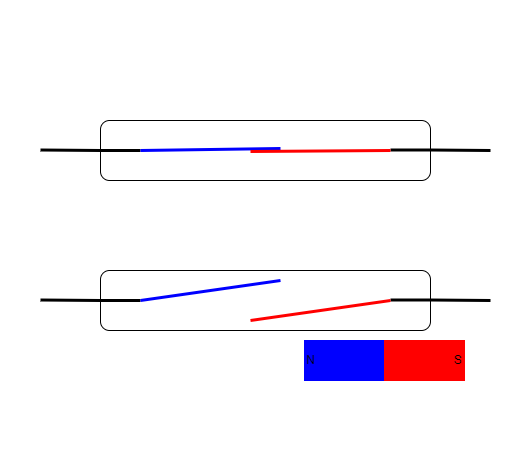
\includegraphics[width=.7\linewidth]{fig/GY-521/zasada_dzialania/zasada_dzialania.png}
% \caption{}
% \label{fig:sub3}
% \end{figure}
% \vspace{0.3cm}

% \begin{figure}[H]
% \centering
% \begin{subfigure}{.5\textwidth}
%   \centering
%   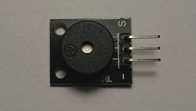
\includegraphics[width=.8\linewidth]{fig/GY-521/zdj_modułu/widok_z_gory_bok.jpg}
%   \label{fig:sub1}
%   \caption{Zdjęcie modułu GY-521}
% \end{subfigure}%
% \begin{subfigure}{.5\textwidth}
%   \centering
%   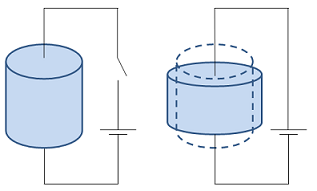
\includegraphics[width=.8\linewidth]{fig/GY-521/zasada_dzialania/piezoelectric_inverse_effect.png}
%   \label{fig:sub2}
%   \caption{Odwrotny efekt piezoelektryczny}
% \end{subfigure}
% %\caption{Połączenie elektryczne}
% \label{fig:test}
% \end{figure}
\begin{document}

%% Strona tytułowa %%
\mainpage{{GY-521/zdj_modułu/tytulowa.jpg}}
\newpage

\section{Opis elementu} \addcontentsline{toc}{section}{Wstęp}
Moduł GY-521 zawiera w sobie dwa główne elementy - żyroskop (do pomiaru prędkości kątowej) i akcelerometr (do pomiaru przyspieszenia). Oba te czujniki są 3-osiowe, co powoduje, że sam moduł staje się narzędziem pomiarowym o 6 stopniach swobody (6DOF). Swoje działanie czujniki bazują na technologii MEMS (eng. Micro Electro-Mechanical System), co oznacza, że pomiary są wykonywane poprzez układ elektryczno - mechaniczny. Zasadę działania MEMS przedstawiono na rysunkach poniżej.

\begin{figure}[H]
\centering
\begin{subfigure}{.5\textwidth}
  \centering
  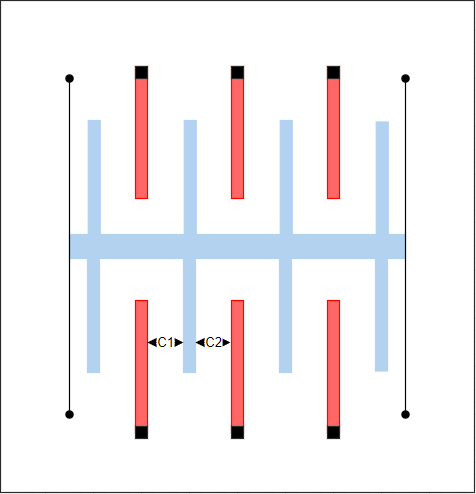
\includegraphics[width=.8\linewidth]{fig/GY-521/zdj_modułu/mems_baza.PNG}
  \label{fig:sub1}
  %\caption{}
\end{subfigure}%
\begin{subfigure}{.5\textwidth}
  \centering
  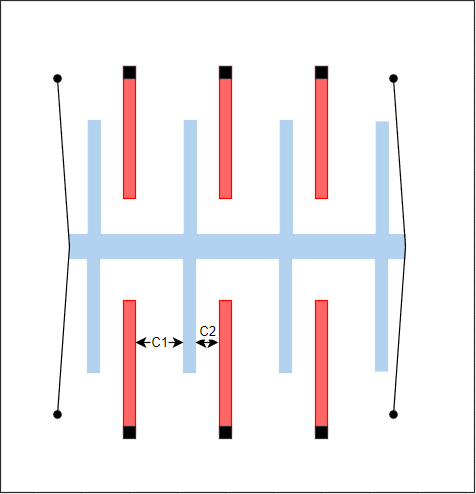
\includegraphics[width=.8\linewidth]{fig/GY-521/zdj_modułu/mems_zmiana.PNG}
  \label{fig:sub2}
  %\caption{Odwrotny efekt piezoelektryczny}
\end{subfigure}
\caption{Na obrazku po lewej została pokazana pozycja wyjściowa, czerwonym kolorem zaznaczono nieruchome płytki, służące za punkt referencyjny, niebieskim - zamontowany na sprężynach zestaw płytek.}
\label{fig:test}
\end{figure}

W trakcie poruszania układu, wzdłuż danej osi, z pewnym przyspieszeniem, na masę zamontowaną na sprężynach działa siła, która powoduje zmianę położenia płytek niebieskich względem czerwonych (w przypadku żyroskopu siłą odpowiedzialną za zmianę położenia niebieskiego zestawu płytek jest siła odśrodkowa). W konsekwencji zmienią się pojemności zaznaczone jako C1 i C2. Zostanie to zarejestrowane przez układ, co po odpowiednim przekształceniu danych, może zostać przekazane dalej jako wartości w $^\circ/sec$ (dla żyroskopu) lub $\frac{m}{s^2}$ (dla akcelerometru). Dane te są wstępnie przetwarzane przez układ DMP (eng. Digital Motion Processor), który zawarty jest w module i powoduje przyspieszenie pracy, a także odciążenie obliczeniowe mikrokontrolera, do którego podłączony jest GY-521.

\subsection{Opis modułu}
Moduł GY-521 zbudowany jest z zestawu podstawowych elementów elektrycznych (kondensatorów, rezystorów, diody LED), układu MPU6050 (zawierającego w sobie opisywane wcześniej akcelerometr i żyroskop oraz termometr cyfrowy), regulatora napięcia serii XC6204 i zestawu pinów. Sam moduł, dzięki posiadaniu pomocniczej magistrali $I^2C$ (eng. Auxiliary $I^2C$, piny XDA i XCL) umożliwia także podłączenie zewnętrznego magnetometru w celu poprawienia identyfikacji położenia modułu względem Ziemii, a dzięki pinowi AD0 możliwe jest wykorzystanie dwóch (lub więcej) MPU6050 w ramach jednej magistrali $I^2C$ poprzez wprowadzenie różnowartościowych adresów (stan AD0 odpowiada wartości LSB w 7-bitowym adresie slave MPU6050). MPU6050 pozwala również na zaprogramowanie filtru Kalmana w celu redukcji szumów.

\vspace{0.3cm}
\begin{figure}[H]
\centering
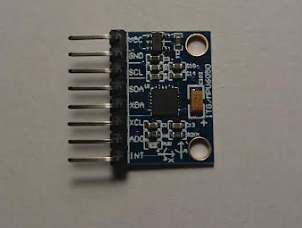
\includegraphics[width=.5\linewidth]{fig/GY-521/zdj_modułu/zdjecie_gy521.PNG}
\caption{Zdjęcie modułu GY-521}
\label{zdj_2}
\end{figure}
\vspace{0.3cm}
\vspace{0.3cm}
\begin{figure}[H]
\centering
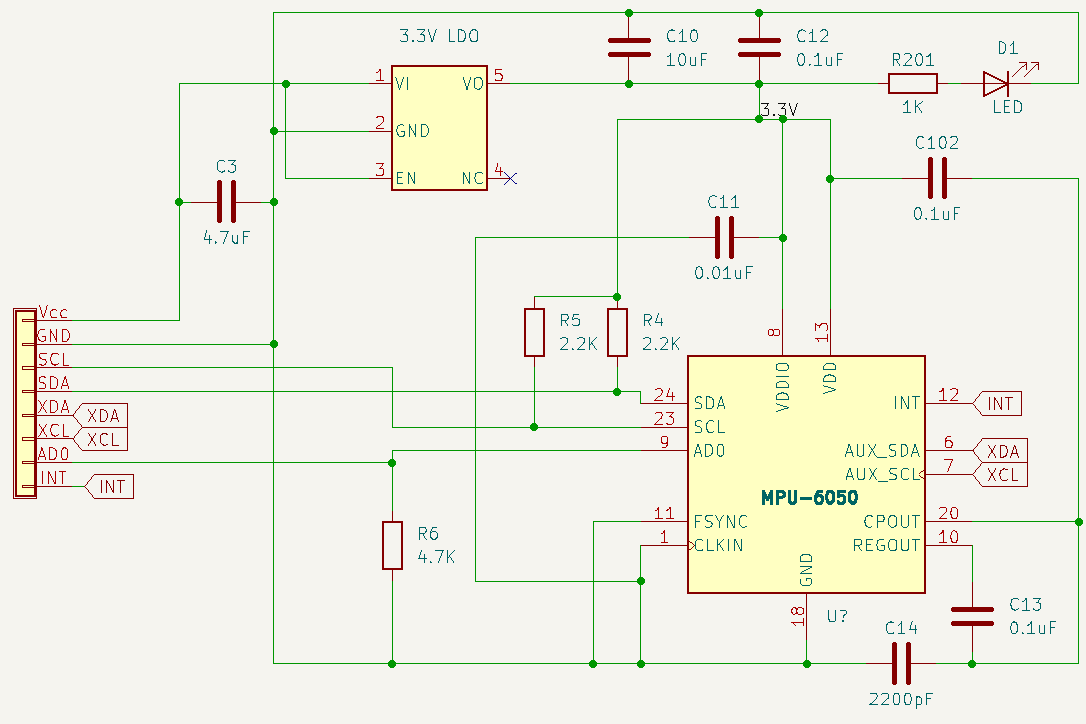
\includegraphics[width=.9\linewidth]{fig/GY-521/zdj_modułu/schemat.PNG}
\caption{Schemat elektryczny GY-521}
\label{fig:sub3}
\end{figure}
\vspace{0.3cm}

\subsection{Zastosowania}
Moduł GY-521, dzięki posiadaniu 6DOF, można użyć jako jednostkę pomiarową IMU (eng. inertial measurement unit), które daje możliwość pomiaru przyspieszenia liniowego i kątowego wzdłuż 3 osi układu odniesienia. Pozwala to na wykorzystanie go w urządzeniach wymagających informacji o wszystkich 6 stopniach swobody np. w ramionach robotycznych, robotach samobalansujących się lub dronach. Poza tym znajdzie on użytek w każdym peryferium wymagającym użycia akcelerometru lub żyroskopu (np. czujnik przechylenia)


\newpage
\hypersetup{
    colorlinks=true,
    linkcolor=blue,
    filecolor=magenta,      
    urlcolor=cyan,
    pdftitle={Overleaf Example},
    pdfpagemode=FullScreen,
    }
\section{Użycie czujnika}
Moduł GY-521 bazuje na wymianie danych z mikrokontrolerem na podstawie protokołu $I^2C$ (synchronicznej, dwukierunkowej magistrali szeregowej bazującej na dwóch liniach danych - SDA, która służy do przesyłania danych i SCL, linii zegarowej, która informuje o tym kiedy zaczyna się i kończy dany bit). W celu pokazania jego działania, został on podłączony odpowiednio do pinów zasilających i pinów odpowiadających za komunikację po magistrali $I^2C$.
\vspace{0.3cm}
\begin{figure}[H]
\centering
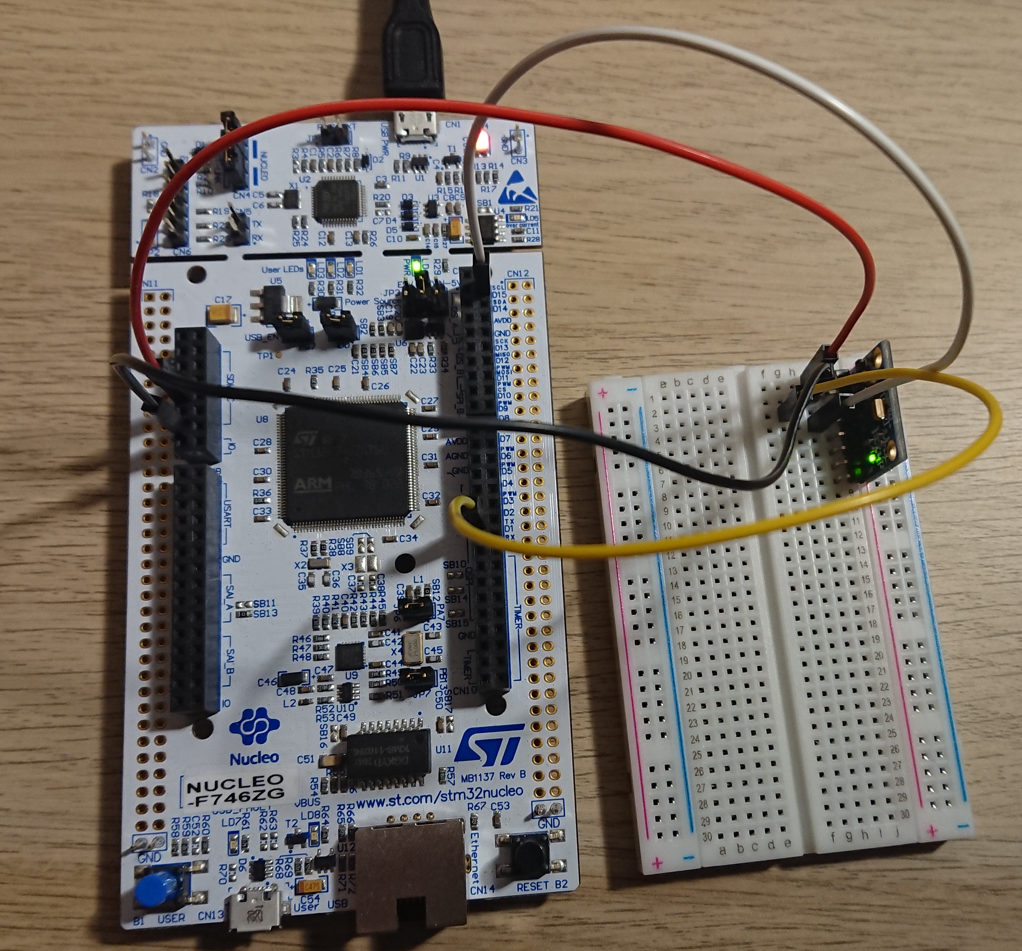
\includegraphics[width=.7\linewidth]{fig/GY-521/działanie_ukladu/podlaczenie.PNG}
\caption{Podłączenie GY-521 do płytki STM32. Widać zieloną diodę informującą o tym, że moduł jest zasilany.}
\label{fig:sub3}
\end{figure}
\vspace{0.3cm}
Następnie, skonfigurowano w środowisku CubeIDE odpowiednio działanie magistrali $I^2C$ oraz napisano odpowiedni kodu na postawie zewnętrznej biblioteki, który umożliwiał sprawdzenie pochylenia czujnika lub jego obrotu (skorzystano z konwencji kątów RPY. Na czujniku narysowane są orientacje dwóch z 3 osi (X i Y, widać to na Rys.\ref{zdj_2} na samym dole czujnika, koło pinu INT) co pozwoliło na odpowiednią interpretację wyników podawanych przez czujniki modułu.
\vspace{0.3cm}
\begin{figure}[H]
\centering
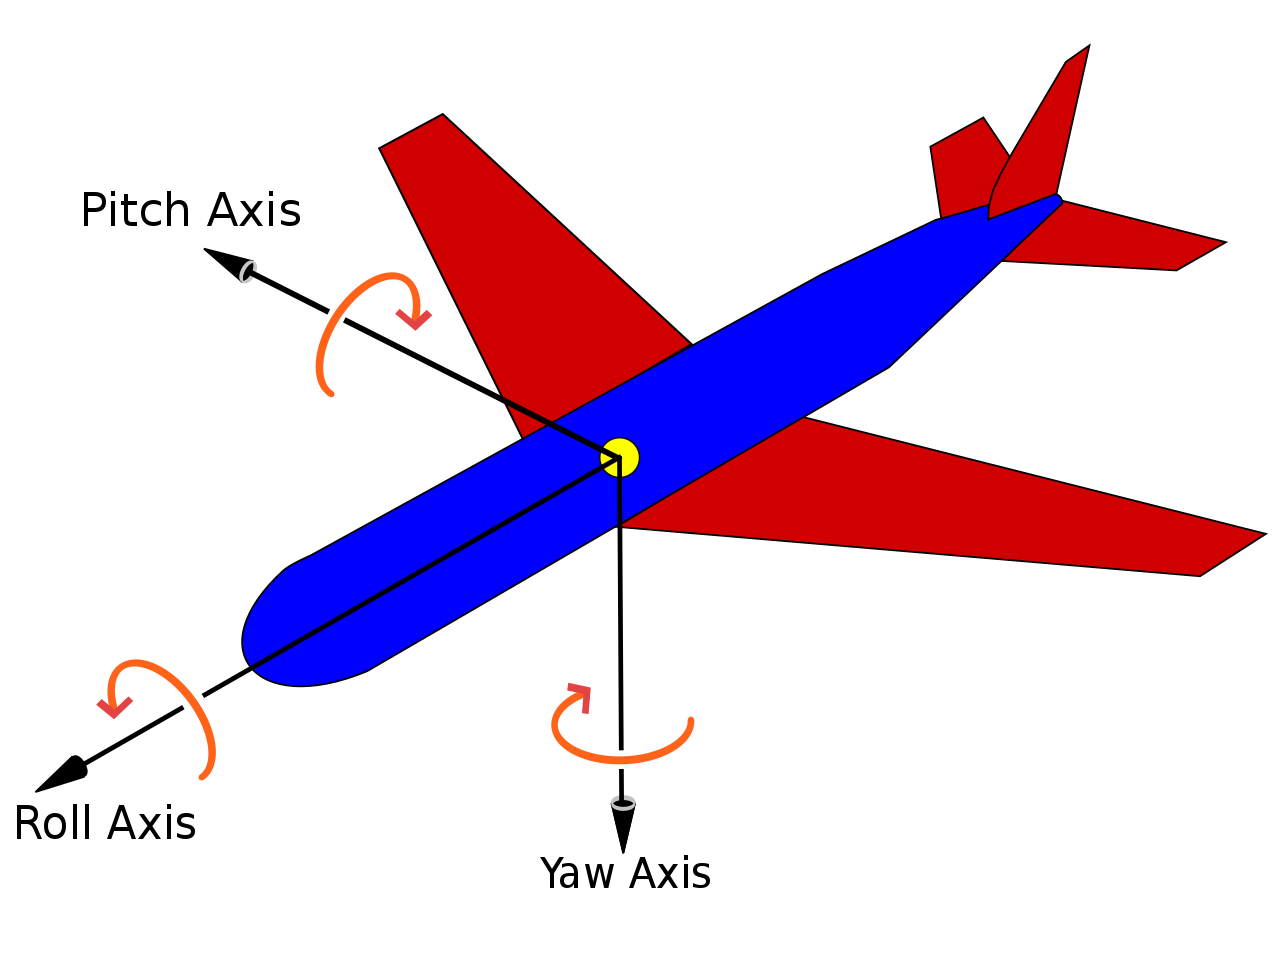
\includegraphics[width=.7\linewidth]{fig/GY-521/działanie_ukladu/Yaw_Axis_Corrected.png}
\caption{Kąty RPY, w celu sprawdzenia działania GY-521 skorzystano jedynie z Roll i Pitch}
\label{fig:sub3}
\end{figure}
\vspace{0.3cm}
\vspace{0.3cm}
\begin{figure}[H]
\centering
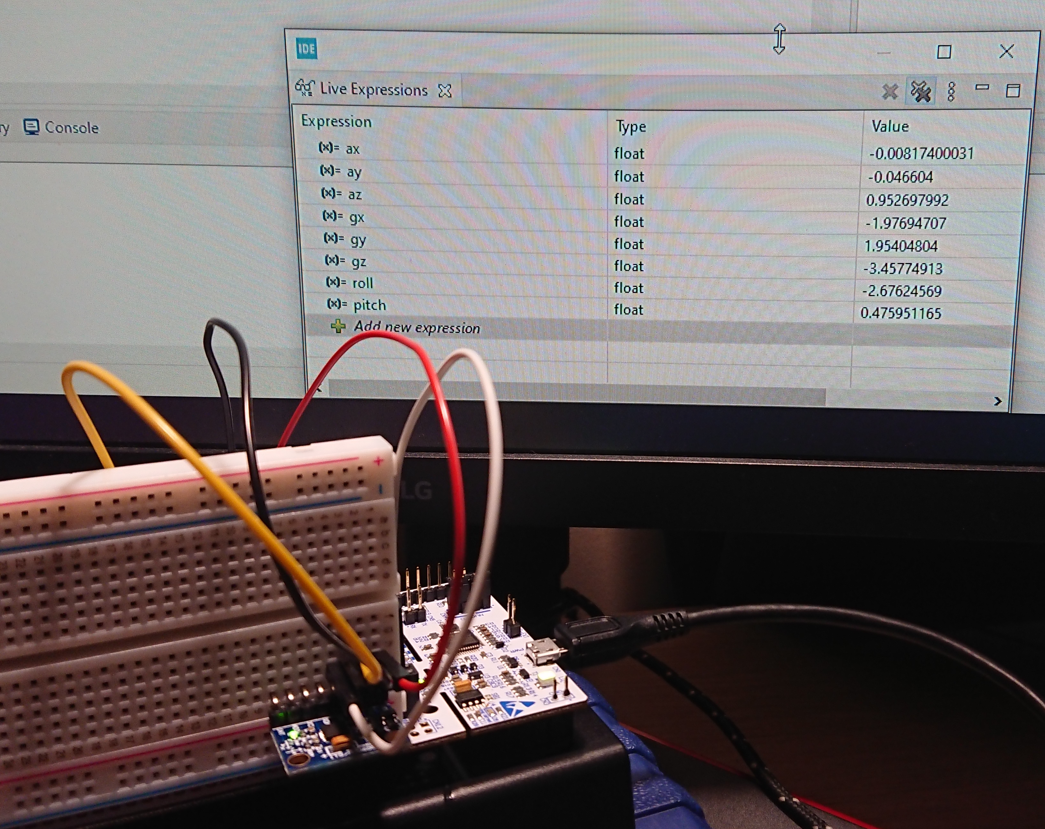
\includegraphics[width=.9\linewidth]{fig/GY-521/działanie_ukladu/base_pos.PNG}
\caption{Czujnik ułożony prawie prostopadle do podłoża, Roll i Pitch bliskie wartościami $0^\circ$}
\label{fig:sub3}
\end{figure}
\vspace{0.3cm}
\vspace{0.3cm}
\begin{figure}[H]
\centering
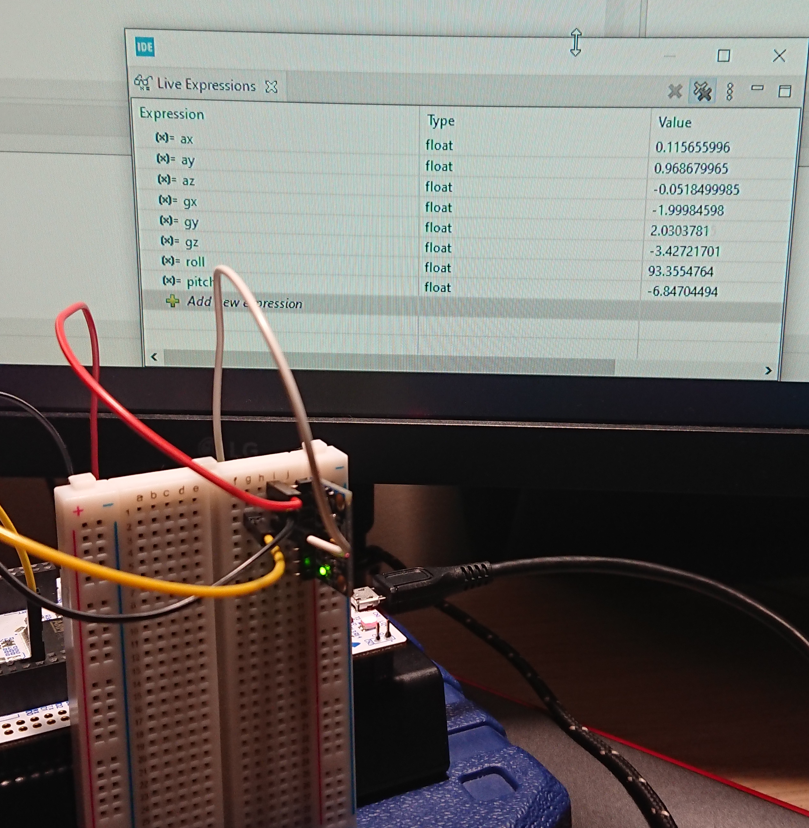
\includegraphics[width=.9\linewidth]{fig/GY-521/działanie_ukladu/not_base.PNG}
\caption{Czujnik obrócony wokół osi własnej X czujnika o ok. $90^\circ$, co widać na podstawie wartości Roll.}
\label{fig:sub3}
\end{figure}
\vspace{0.3cm}
Na powyższym zdjęciu można także zauważyć działanie akcelerometru. Wartość ''ay'' określa przyspieszenie w osi Y, która w tym ułożeniu jest prostopadła do podłoża, oznacza to, że na akcelerometr w tej osi działa przyspieszenie równe w przybliżeniu wartości przyspieszenia ziemskiego (na podstawie odczytów i przeskalowania wartość 1 dla zmiennych ax, ay i az to wartość równa przyspieszeniu ziemskiemu $g\approx9.81\frac{m}{s^2}$)


\printbibliography[heading=bibintoc]

\end{document}